\documentclass{instructions}

\usepackage{xspace}

\newcommand{\git}{\texttt{git}\xspace}
\newcommand\bs{\char`\\}

\title{Practical 1: Software engineering for roboticists}
\date{\today}

\summary{
Headfirst in software engineering for robotics: you will discover and
put to use several tools (the Linux command-line, SSH, GIT,...) that
make the core of the software toolkit of roboticists.
}

\objectives{
At the end of the practical, you should know how to:

\begin{itemize}
    \item create a GitHub account
    \item know what Markdown is and use it to write your first entry in your lab
        journal
    \item know what GIT is, and use it to track the changes to your lab
        journal
    \item use the Linux terminal and SSH to connect to a remote robot
    \item write a simple Python program to get the robot to speak
    \item use GIT to add your Python code to your repository and track it
\end{itemize}
}

\challenges{

    \begin{itemize}
        \item Getting acquainted to the Linux command-line;
        \item Create a mental model of how
    code is managed;
        \item Hack into a robot!
    \end{itemize}
}

\begin{document}

\maketitle


\note{
    Please note that \textbf{you are required to attend all the laboratory
practical sessions}.

You are required to write a short report on each of the practical
you attend, and add it to your \textbf{lab journal} (cf below). This should describe:

\begin{itemize}
    \item The task or problems you were asked to solve.
    \item An explanation of your solution.
    \item Your results, findings and insights.
\end{itemize}

\begin{center}
    \textbf{The coursework is assessed and worth 60\% of your final mark for this
    module.}

    Also, you work in pairs for the practical sessions but
    submit a report \textbf{INDIVIDUALLY}.
\end{center}
}


%%%%%%%%%%%%%%%%%%%%%%%%%%%%%%%%%%%%%%%%%%%%%%%%%%%%%%%%%%%%%%%%%%%%%%%%%%%%%%%%%%%%%%%%%%
\intro

All the software-related bits of the practicals will take place on Linux. To
start with, ensure your computers are booted on a Linux session.


\part{Your lab journal}


Good news, everyone: no 'final report' to write for the ROCO222 practicals.
Instead, you keep, week after week, a \textbf{lab journal} that contains
everything you have attempted, found out, learnt that week.

\note{
    Your \textbf{individual} lab journal \textbf{is assessed}: make sure you
    enrich it with pictures of what you have built and diagrams whenever it is
    useful.

    Check as well the \textbf{Objectives} listed at the top of the instruction
    sheets every weeks: make sure your lab journal discuss all the targets.
}

\step{Write your first Markdown document}

Look on the Web what is Markdown, and start your lab journal using the Markdown
syntax. In this first journal entry, describe what Markdown is about, and write
down the key syntax rules. For now, you can write a single document for the two
of you. Name it \texttt{journal.md}.

\note {
Find and open \texttt{gedit} to edit text files on Linux. As soon as you save
your file with the \texttt{.md} extension, \texttt{gedit} recognises it as a
Markdown file and conveniently highlights the syntax.
}

\step{Command-line 101}

Find and open a terminal (also called \emph{console}).

Try the following commands and briefly write down in your lab journal what they do.
If something is not clear, \texttt{man <command>} should provide you with some
help (\texttt{man} stands for \emph{manual}).

\begin{shcode}
$ ls
$ cd /tmp
$ cd $HOME # what are those things starting with '$'?
$ mkdir
$ echo "Hello" > hello.md
$ cat hello.md
$ cp hello.md hello-again.md
$ mv hello-again.md hello-hello.md
$ rm hello.md
$ rm -rf # be careful with that one!
$ cat /proc/cpuinfo # is 'cpuinfo' a file??
\end{shcode}


Create a \texttt{roco222} subdirectory in your \emph{home} directory, then one
subdirectory for each of you, and finally a sub-subdirectory named
\texttt{lab-journal}. Make a copy of your lab journal in each of
these directories.

\note{
    This step could easily be done with the file manager. But soon enough, you
    will be working remotely on robots or dev boards with no graphic interface.
    Better to get used to the console!
}

\step{Create a GitHub account}

\git is a widely-used tool to manage code and other text-based documents. You
will use it to manage your lab journal.

GitHub is a (proprietary) online platform to share \git repositories. While not
required to use \git, we will make use of GitHub today. If you do not already
have an account, create one from the website: \url{https://github.com}.

\step{Your first git repository}

Initialise the each of your \git \textbf{repositories} by navigating to each of
the directories you created. Type \sh{git init} in there. The name of the
directory is the name of your repository.

That's it: a \git repository is a regular directory, with one
special item: an hidden \texttt{.git/} directory that stores all the
\textbf{objects} \git manipulates (mainly binary blobs representing files or
parts of files).

\more{
Type \sh{ls -al} to get a detailled list of all files in a directory, including hidden files.
Try to figure out what the different informations on each line mean, and add
it to your lab journal.
}

As this is the first time you are using \git, you need to tell it what is your
name and what is your email address, so that all your changes are
effectively attributed to you. In each of the repositories, type:

\begin{shcode}
$ git config user.name "Firstname Surname"
$ git config user.email "<email>"
\end{shcode}

\step{Your first commit}


We are going to \textbf{commit} the current state of your lab journal: since
the file \texttt{journal.md} is
not yet known to \git, first \textbf{add it}: \sh{git add journal.md}, and
then create a new \textbf{commit} with \sh{git commit}.

\git will ask you for a
commit message (a commit message is made of a mandatory one-line \emph{summary} --
usually maximum 72 characters long -- and a longer, optional, \emph{description} that explains
in greater details what this commit is about).

The commit summary must be concise yet must describe accurately the content of
the change. For instance, ``Created journal -- initial report on Markdown syntax''.

\note{
    You can use \sh{git commit -m"commit message"} to directly create a commit
    with a commit message.
}

By typing \sh{git log}, you can see the
history of changes in your repo. \texttt{gitk} is another
convenient way to display in a graphical way the history of the repo.

\more{
One of the first steps after creating a new repository is to add a
\texttt{README} file that describes briefly the content of the repository:
create such a file and briefly describes what this repository is about --
reporting on the ROCO222 practical work in a journal-like fashion.

It is common practise to write \texttt{README}s using the \textsc{Markdown}
syntax as well -- your file will then be named \texttt{README.md}.
}

\step{Version tracking}

Add a new entry in your journals describing what you have just learnt about
\git.

Using \sh{git status}, review the changes and commit them (\sh{git
commit <your file>}, choosing an appropriate commit message.

\step{Going social}

Until now, you have only worked on a \textbf{local} \git repository: this is a
perfectly legitimate use of \git. As a \textbf{distributed version control
system} (DVCS), \git is meant to support a wide range of code workflows,
including purely local workflows: if you do not need to share your code over
Internet, why would you need an Internet connection to benefit code versioning?

However, \git is particularly powerful when working in groups: the core idea is
that each participant own a full copy of a repository, and exchanges commits
through \textbf{pushes} (to send commits to others) and \textbf{pulls} (to get
commits from others). As you can see on the figure below (and contrary to
traditional VCS like SVN), you \textbf{do not
need to use a central server} (but you can!): \git is distributed, each
participant own a full, autonomous copy of the repository and can obtain
(\emph{pull}) commits from any other participant.

\begin{center}
    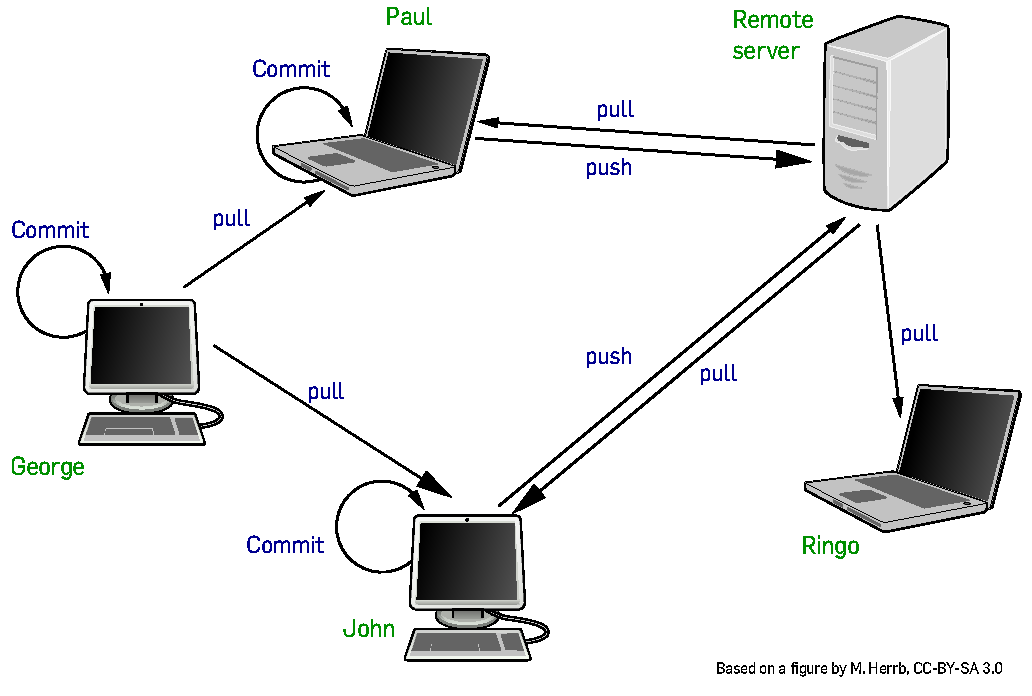
\includegraphics[width=0.8\linewidth]{figs/distributed-git.pdf}
\end{center}

Distant repositories can be on a remote Internet server like GitHub, on your
colleagues' computers,
or even on a USB stick that you carry over with you. \git calls them
\textbf{remotes}. You can add as many remotes as you want to your local
repository by giving them names.

Often, you will have one main remote, which is traditionally called
\texttt{origin} (but it's up to you to choose a different name!).



Add GitHub as a remote repository to your local \git repository.

First create an empty repository on GitHub:

\begin{center}
    
\includegraphics[width=0.3\linewidth]{figs/github-new.png}
\end{center}

Name it after your local repository (not mandatory, but convenient), and do
\textbf{not} check the checkbox ``Initialize this repository with a README''
since you already have one.

Then, add this remote to your local repository, and \textbf{push} your changes
online:

\begin{shcode}
$ cd <REPO DIR> # for instance $HOME/roco222/joe/journal
$ git remote add origin https://github.com/<account>/<repo>.git # add a remote called origin
$ git push -u origin # push all your local commits to GitHub
\end{shcode}


\more{
    In this example, you use the \texttt{https} protocol as \textbf{transport}
    between the remote server and your local repository. This requires you to
    type you login and password every time.
    
    \git is however often used with \texttt{ssh} as transport. No password is
    required in that case (it transparently uses your \texttt{ssh} keys to establish
    an encrypted connection to the remote server). You can easily configure
    your GitHub account to use \texttt{ssh}. Read the documentation here:\\
    \url{https://help.github.com/articles/generating-ssh-keys/}
}


If you refresh the GitHub interface in your browser, you should be able to see
your journal online.

Next time you want to send your changes to the remote server, just do:

\begin{shcode}
$ git push
\end{shcode}

\more{

    How to retrieve changes from the server, then? When you're back at home, go
    and read \url{http://rogerdudler.github.io/git-guide/}.

    Do it. Really. You will need it.
}

\important{
From now on, track all the changes to your journal using \git.

\textbf{Coursework will be submitted by provinding a link to your GitHub
repository. The number and regularity of commits will count toward your
mark.}
}


\part{Hack into a robot}

Quite simple really. Figure out a way to log into the robot. Those two bits of
information should be sufficient: it's an Aldebaran's
Nao and its name is 'chapman'.

Obviously, you are not allowed to physically
interact with it :-)

Once logged onto the robot, the following Python program will get the robot to
say something:

\begin{pythoncode}
from naoqi import ALProxy
tts = ALProxy("ALTextToSpeech", "localhost", 9559)
tts.say("I've hacked you, robot!")
\end{pythoncode}


The first group who gets the robot to speak wins a very nice robot sticker!

Some further keywords to google for:

\begin{shcode}
.local domain
howto ssh
nano editor
running python program console
\end{shcode}

\section{Complete the lab journal}

Complete your lab journal with your experience connecting to the robot, commit
and push it to your \git repo. Include as well the Python script, either as a
separate Python file, or directly in your Markdown document (research first how to
include code snippets in a Markdown document).

\important{
    Always push all your changes before leaving the lab: these computers are
    shared, and we can not guarantee that your work will still be there next
    week!
    
    (it should, though...)
}


\part{Next steps}


\section{Getting familiar with git}

\git is a large system that may appear complex at first sight. Take some time to
get used to it: becoming familiar with \git will be soon rewarding! and do not
hesitate to ask questions during the coming weeks.

This tutorial did not introduce many concepts like \textbf{pull requests}, \textbf{branches},
\textbf{conflicts} or \textbf{rebase}. If you want to learn more on \git, here a
few resources:

\begin{itemize}
    \item Many \git \emph{cheatsheets} exist. Tower has a good one
        (\url{http://www.git-tower.com/blog/git-cheat-sheet/}), GitHub as well
        (\url{https://help.github.com/articles/git-cheatsheet/}), and a nice
        interactive cheatsheet is there:
        \url{http://ndpsoftware.com/git-cheatsheet.html}
    \item \emph{git from the bottom up} is a great (and esay) reading to understand how
        \git actually work. As a matter of fact, most \git commands become evident once you know how they are
        built. \url{https://jwiegley.github.io/git-from-the-bottom-up/}
\end{itemize}


\section{Installing git at home}


If you want to install \git on your system, here the brief
summary:

\git installation depends on your operating system. If running Linux,
everything is simple, just install \git with your distribution's
favorite package manager (on Debian/Ubuntu,
\texttt{sudo apt install git}).

On Windows/MacOSX, we recommend you to use the GitHub official app, that takes
care of properly configuring \git for your system, and also provide an
easy to use user interface (but obviously, an ``easy to use'' interface also means
that it hides things from your eyes, and makes the underlying mecanisms harder to
understand. Anyway...) Head to \url{https://desktop.github.com/}

\note{
Once installed, the Windows GitHub app also provides a link to the Windows
shell, conveniently configured to work with Git. We encourage you to make use of
it and use the command-line based instructions below.  }

With \git installed on your own machine, you can \textbf{clone} your ROCO222
repository to get a local copy of it at home, and synchronise it with your work
at the uni.

\end{document}
